\documentclass[11pt,a4paper]{article}
\usepackage[margin=2.2cm]{geometry}
\usepackage{graphicx}
\usepackage{booktabs}
\usepackage{longtable}
\usepackage{amsmath,amssymb}
\usepackage{hyperref}
\usepackage{caption}
\usepackage{enumitem}
\usepackage{xcolor}
\graphicspath{{figures/}}
\hypersetup{colorlinks=true,linkcolor=blue!50!black,urlcolor=blue!50!black}
\title{Can GPT-6 Astra Do the Physics?\\Engineering Drawings that Require Computed Results}
\author{SVG Patch Lab --- generation eval \texttt{engineering\_v2\_physics}}
\date{11 September 2026}

\begin{document}
\maketitle

\begin{abstract}
The first evaluation (\texttt{engineering\_v1}) showed \texttt{gpt-6-astra} drafts complex engineering drawings essentially without error. This second set asks a harder question: can the model \emph{compute the physics} the drawing is supposed to show, and where does it need a field solver (FEM/PINN) behind it? Twenty prompts require labelled results from solid mechanics, heat transfer, fluids, vibration and circuits; ground truth is computed independently by script and matched against the drawing's labels with a tolerance check. Result: \textbf{all 16 closed-form problems are numerically correct}, and for the two field problems with analytic solutions (Laplace's equation on a square, potential flow past a cylinder) the drawn curves \emph{lie on the exact solution} --- isotherm positions match a Fourier series to three decimals, and the stream function is constant along every streamline to under 1\,\%. The two field problems \emph{without} a closed form are where it breaks: the finite-plate capacitor's fringing field has physically impossible topology (closed electric field lines), and the L-bracket von Mises map is self-declared ``illustrative''. That boundary --- analytic vs.\ non-analytic fields --- is exactly where an FEM/PINN solver must supply the field and the model should only render it. Run cost: \$4.81 at \texttt{reasoning\_effort=medium}.
\end{abstract}

\section{Setup}
\begingroup\raggedright
\begin{description}[style=nextline,leftmargin=2em]
  \item[Model] \texttt{gpt-6-astra} via \url{https://api.openai.com/v1/chat/completions}, \texttt{reasoning\_effort=medium}, \texttt{max\_completion\_tokens=16000}, no sampling parameters. One user message, no tools.
  \item[Prompt set] \texttt{configs/prompts/engineering\_v2\_physics.json}, generated by \texttt{scripts/make\_physics\_prompts.py} so that every expected value is computed (closed-form formula in code), never typed. 16 \emph{closed-form} problems and 4 \emph{field} problems.
  \item[Checks] The harness's new \texttt{number\_near} check scans every \texttt{<text>} label for a number within a relative tolerance (default 2\,\%) of the expected value, accepting equivalent unit/scale forms (e.g.\ $48\,182\,172$\,mm$^4$ or $48.2\times10^6$\,mm$^4$). 124 checks in total. Field problems get one anchor value each plus a post-hoc quantitative comparison against the analytic solution.
  \item[Rendering] Figures via macOS QuickLook from the raw SVG output.
  \item[One ground-truth correction] The L-bracket beam-theory check was initially written with the wrong section width (40 instead of 80\,mm) and lever arm; Astra's 122\,MPa ($Z=bt^2/6$, $h=52$\,mm) was correct and the ground truth was fixed and the run rescored offline (\texttt{--rescore}, no model calls).
\end{description}
\endgroup

\section{Results}
\subsection{Aggregate}
\begin{center}
\begin{tabular}{lr}
\toprule
Prompts (closed form / field) & 20 (16 / 4) \\
Valid SVG & 20/20 \\
Closed-form problems numerically correct & 16/16 \\
Field problems: analytic solution reproduced & 2/2 \\
Field problems: non-analytic, physically faithful & 0/2 \\
Structural + numeric checks passed & 124/124 (after the ground-truth fix) \\
Input / output tokens & 5175 / 95248 \\
\quad of which reasoning & 30684 \\
Mean output tokens / latency per drawing & 4762 / 93\,s \\
Total cost & \$4.81 \quad (\$0.241 / drawing) \\
\bottomrule
\end{tabular}
\end{center}

\subsection{Per-prompt}
{\small
\begin{longtable}{llrrrll}
\toprule
Prompt & Kind & Out tok & Reason. & s & Checks & Verdict \\
\midrule
\endhead
\texttt{cantilever\_deflection} & closed form & 3994 & 825 & 76 & 6/6 & Pass \\
\texttt{composite\_wall\_conduction} & closed form & 3456 & 688 & 67 & 6/6 & Pass \\
\texttt{plate\_hole\_kirsch} & closed form & 5218 & 984 & 93 & 7/7 & Pass \\
\texttt{truss\_member\_forces} & closed form & 4246 & 697 & 75 & 6/6 & Pass \\
\texttt{mohr\_circle} & closed form & 4936 & 1537 & 87 & 7/7 & Pass \\
\texttt{cantilever\_mode\_shapes} & closed form & 8507 & 5120 & 189 & 8/8 & Pass \\
\texttt{poiseuille\_profile} & closed form & 3911 & 628 & 66 & 7/7 & Pass \\
\texttt{rc\_bode\_plot} & closed form & 4447 & 1536 & 85 & 7/7 & Pass \\
\texttt{udl\_beam\_shear\_moment} & closed form & 3339 & 477 & 53 & 5/5 & Pass \\
\texttt{pin\_fin\_temperature} & closed form & 4288 & 1024 & 85 & 7/7 & Pass \\
\texttt{euler\_buckling} & closed form & 4163 & 830 & 75 & 6/6 & Pass \\
\texttt{laplace\_plate\_isotherms} & field & 7860 & 5632 & 177 & 4/4 & Exact \\
\texttt{potential\_flow\_cylinder} & field & 6717 & 2495 & 132 & 6/6 & Exact \\
\texttt{ibeam\_shear\_stress} & closed form & 4176 & 1444 & 79 & 6/6 & Pass \\
\texttt{capacitor\_fringe\_field} & field & 5873 & 2560 & 128 & 4/4 & Fail (topology) \\
\texttt{thick\_cylinder\_lame} & closed form & 4556 & 1024 & 85 & 7/7 & Pass \\
\texttt{shaft\_torsion} & closed form & 4894 & 794 & 90 & 6/6 & Pass \\
\texttt{rc\_step\_response} & closed form & 3111 & 853 & 58 & 8/8 & Pass \\
\texttt{lbracket\_von\_mises} & field & 4852 & 1024 & 101 & 5/5 & Illustrative \\
\texttt{dam\_hydrostatic} & closed form & 2704 & 512 & 53 & 6/6 & Pass \\
\bottomrule
\end{longtable}
}

\begin{figure}[p]
  \centering
  
\includegraphics[width=\textwidth]{contact-1.png}\\[6pt]
  
\includegraphics[width=\textwidth]{contact-2.png}
  \caption{All 20 drawings in prompt order.}
\end{figure}

\section{Closed-form physics: 16/16 correct}
Every labelled result matched the independently computed value within tolerance (most to 3--4 significant figures). Beyond the labels, the \emph{curves} are right: the cantilever mode shapes carry the tabulated node positions $x/L = 0.7834$ (mode 2) and $0.5035,\ 0.8677$ (mode 3) (Fig.~\ref{fig:modes}); the Bode plot has the $-3.01$\,dB point, $-45^{\circ}$ phase and $-20$\,dB/decade asymptote at the right places; Mohr's circle is to scale with the correct centre, radius and principal angle. Typical reasoning spend was 500--1500 tokens; the eigenvalue problem took 5120.

\begin{figure}[t]
  \centering
  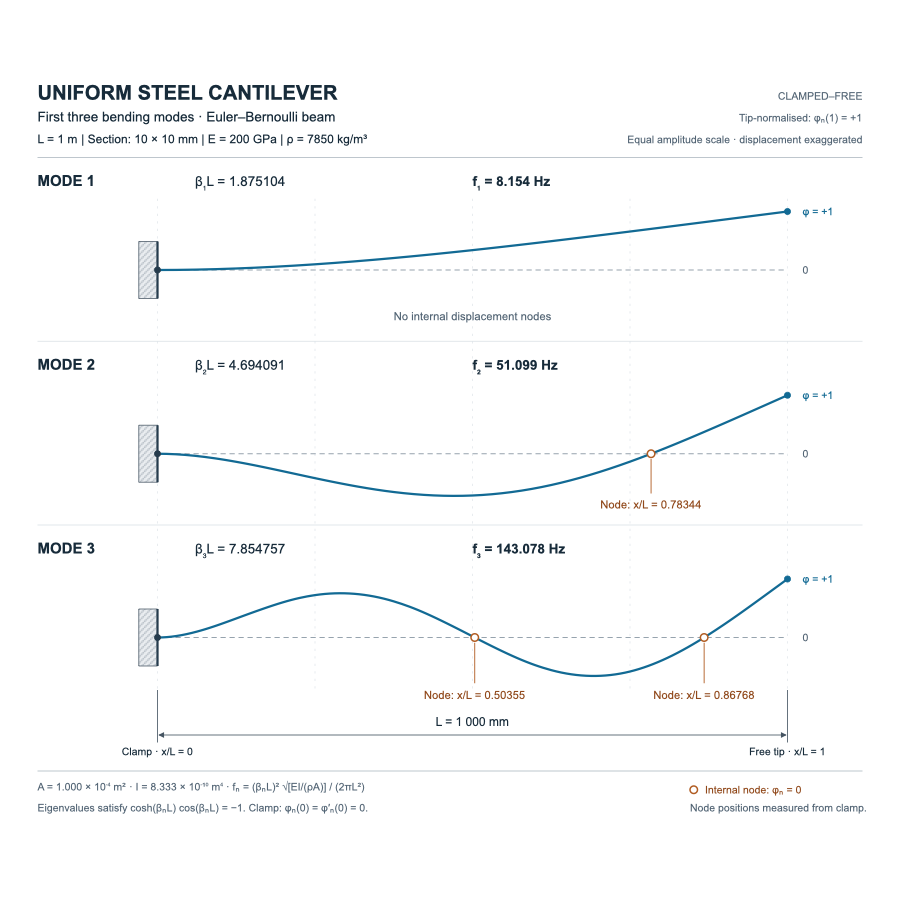
\includegraphics[width=0.58\textwidth]{cantilever_mode_shapes.png}\hfill
  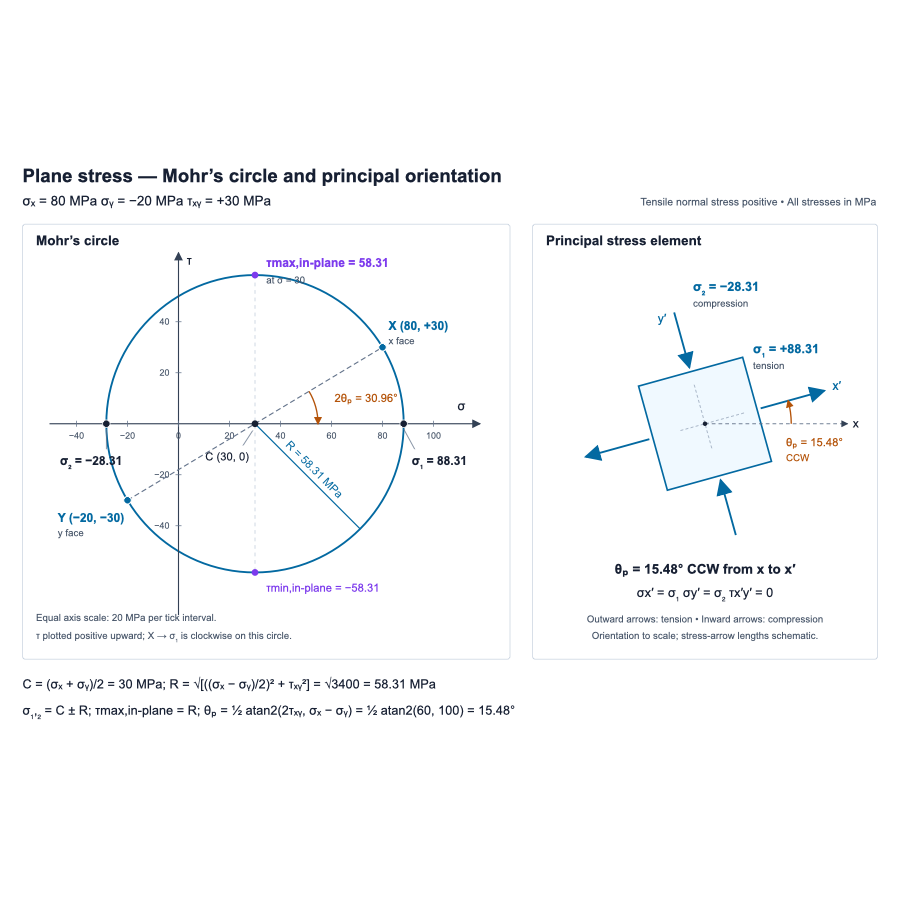
\includegraphics[width=0.40\textwidth]{mohr_circle.png}
  \caption{Left: first three cantilever modes with $\beta_nL$, $f_n$ and node positions --- all exact. Right: Mohr's circle for $(80,-20,30)$\,MPa.}
  \label{fig:modes}
\end{figure}

\section{Field problems: where the line is}
\subsection{Analytic fields --- reproduced exactly}
\textbf{Laplace plate.} The isotherms are cubic B\'ezier chains whose knots sit at fixed $x$. Reading the knot at $x=0.25$ and $x=0.5$ for each isotherm and evaluating the series solution
$T(x,y)=\frac{400}{\pi}\sum_{n\ \mathrm{odd}}\frac{1}{n}\sin(n\pi x)\frac{\sinh(n\pi y)}{\sinh(n\pi)}$ at those points gives the isotherm's own temperature to $\pm0.05$\,$^{\circ}$C in all ten cases; equivalently the position error is $<0.001$\,m on a 1\,m plate (Table~\ref{tab:iso}). The model spent 5632 reasoning tokens and evidently evaluated the series.

\begin{table}[h]
\centering
\begin{tabular}{rrrrr}
\toprule
Isotherm ($^{\circ}$C) & $x$ & drawn $y$ & exact $y$ & $T_{\text{exact}}$ at drawn point \\
\midrule
10 & 0.25 & 0.338 & 0.338 & 10.0 \\
10 & 0.50 & 0.260 & 0.260 & 10.0 \\
20 & 0.25 & 0.527 & 0.527 & 20.0 \\
20 & 0.50 & 0.435 & 0.435 & 20.0 \\
40 & 0.25 & 0.728 & 0.728 & 40.0 \\
40 & 0.50 & 0.648 & 0.648 & 40.0 \\
60 & 0.25 & 0.844 & 0.844 & 60.0 \\
60 & 0.50 & 0.788 & 0.787 & 60.0 \\
80 & 0.25 & 0.928 & 0.928 & 80.0 \\
80 & 0.50 & 0.899 & 0.899 & 80.0 \\
\bottomrule
\end{tabular}
\caption{Drawn isotherm knots vs.\ the exact Laplace solution ($y$ measured from the cold bottom edge).}
\label{tab:iso}
\end{table}

\textbf{Potential flow.} For each of the eight streamline paths, $\psi = U\,y\,(1-a^2/r^2)$ evaluated at every knot is constant to $\pm0.002$--$0.006$ (levels $0.149, 0.304, 0.503, 0.749$ m$^2$/s), i.e.\ the curves are genuine streamlines, not sketched bumps.

\begin{figure}[t]
  \centering
  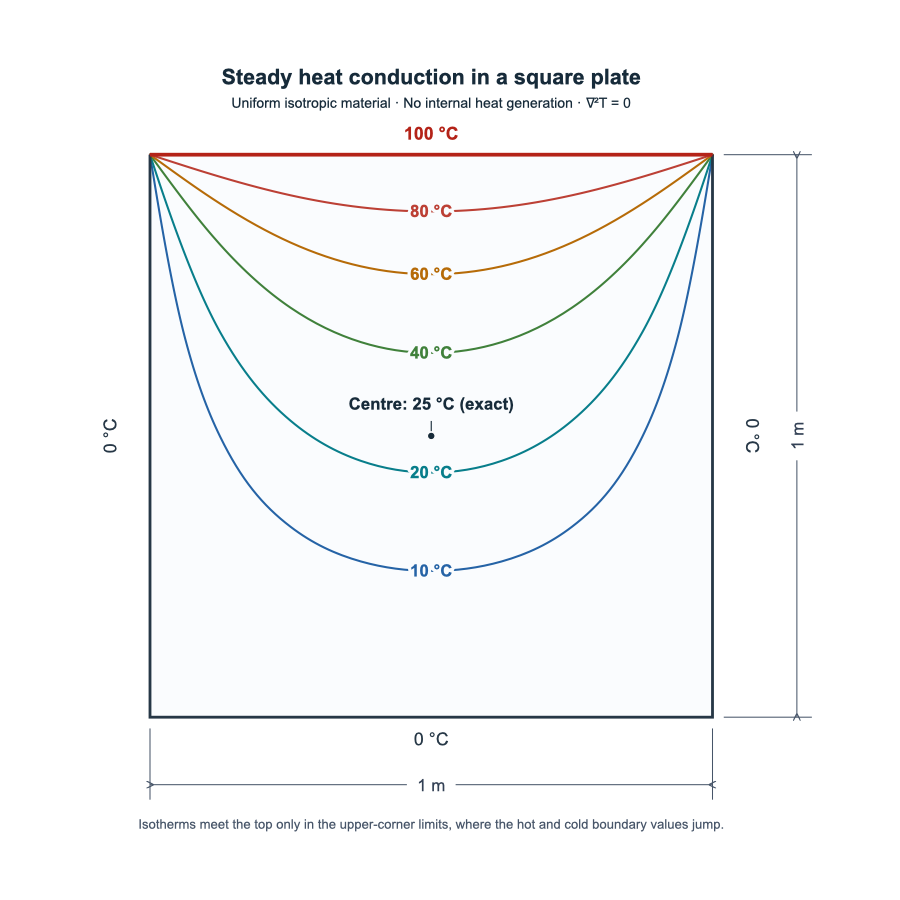
\includegraphics[width=0.46\textwidth]{laplace_plate_isotherms.png}\hfill
  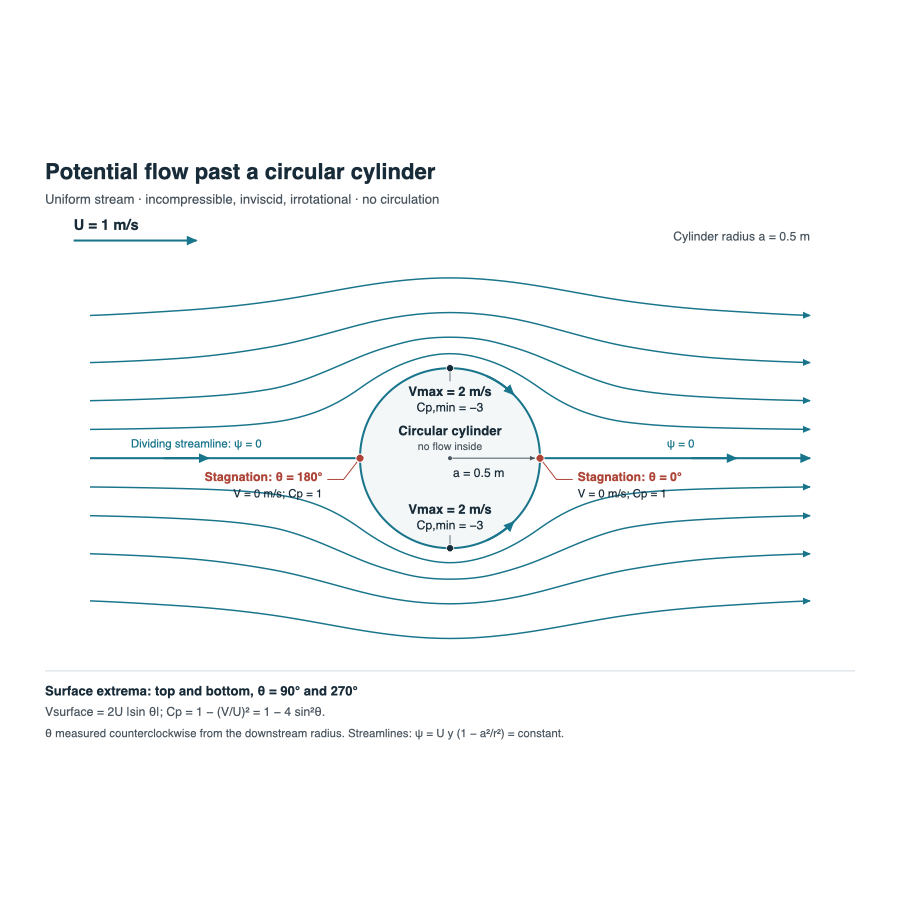
\includegraphics[width=0.52\textwidth]{potential_flow_cylinder.png}
  \caption{Analytic field problems: both drawn from the exact solution.}
\end{figure}

\subsection{Non-analytic fields --- faked}
\begin{description}[style=nextline,leftmargin=1em]
\item[\texttt{capacitor\_fringe\_field}] \textbf{Fail (topology)} --- Field lines at the plate ends drawn as closed circles (impossible for an electrostatic field, $\nabla\times\mathbf{E}=0$); the $\pm25/50/75$\,V equipotentials run off to infinity instead of closing around their plate. Uniform region and $E=10$\,kV/m correct.
\item[\texttt{lbracket\_von\_mises}] \textbf{Illustrative} --- Self-labelled ``illustrative \ldots not a solved FE model''; peak from an assumed $K\approx1.8$ on the beam-theory root stress (122\,MPa, correct). Contour bands are decorative, not a solution.
\item[\texttt{laplace\_plate\_isotherms}] \textbf{Exact} --- Isotherm knots lie on the Fourier-series solution to 3 decimals at all 10 sampled points; centre 25\,$^{\circ}$C.
\item[\texttt{potential\_flow\_cylinder}] \textbf{Exact} --- $\psi=Uy(1-a^2/r^2)$ constant along every streamline to $<1\%$; stagnation points, $V_{\max}=2U$, $C_{p,\min}=-3$ correct.
\end{description}

\begin{figure}[t]
  \centering
  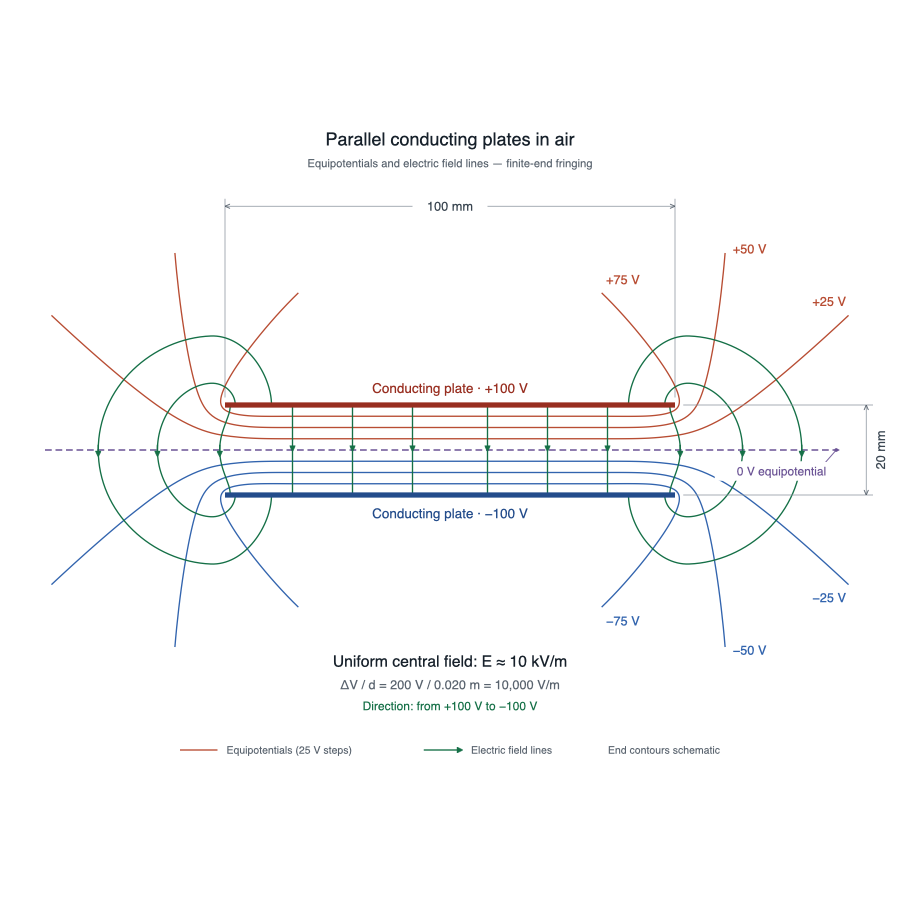
\includegraphics[width=0.50\textwidth]{capacitor_fringe_field.png}\hfill
  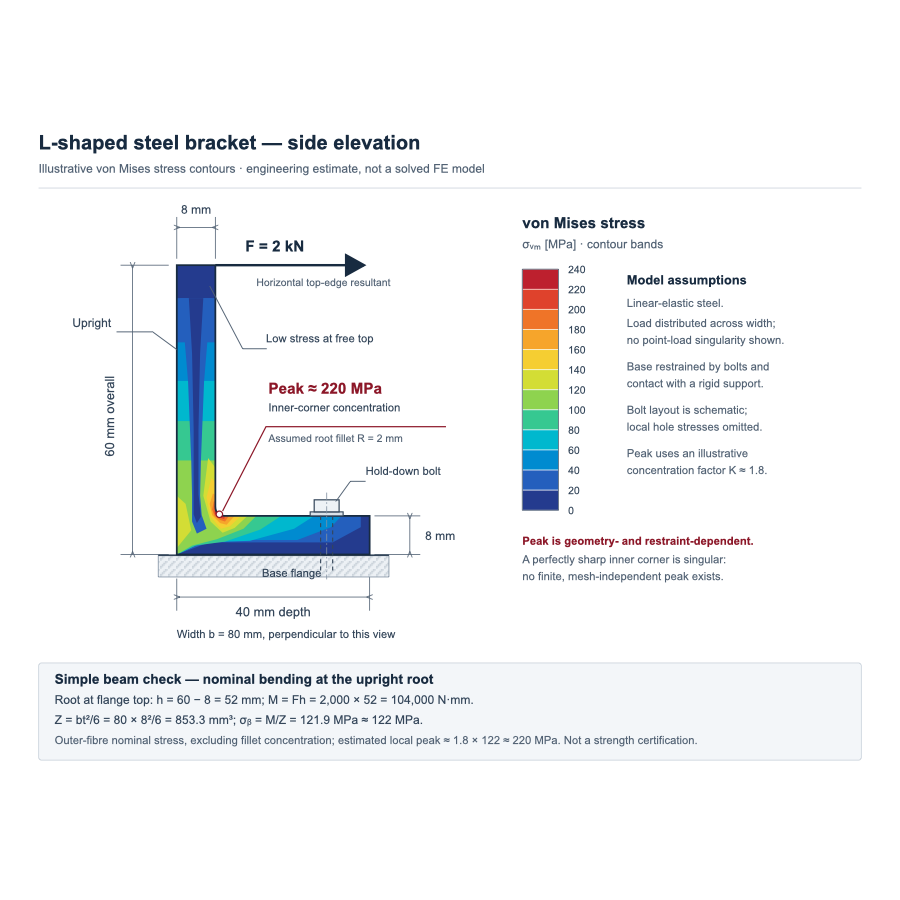
\includegraphics[width=0.48\textwidth]{lbracket_von_mises.png}
  \caption{Left: the fringing field at the plate ends is drawn as closed circular ``field lines'' and the outer equipotentials leave to infinity --- wrong topology for an electrostatic field. Right: an FEA-looking von Mises map that the model itself labels illustrative.}
  \label{fig:fail}
\end{figure}

The pattern is consistent: when a closed-form solution exists the model computes it and draws from it; when the field must be solved numerically it draws a plausible picture and, to its credit, says so (the bracket) --- or does not (the capacitor, where the caption ``end contours schematic'' understates a physical impossibility).

\section{Implications for an FEM/PINN pipeline}
\begin{itemize}
  \item \textbf{Do not spend solver effort on textbook cases.} Beam deflection, 1-D conduction, Lam\'e, torsion, buckling, Mohr, fin equation, Laplace on a rectangle, potential flow: Astra's results are as accurate as the closed form. A solver adds nothing but cost.
  \item \textbf{The solver's job is the non-analytic field.} Finite-plate fringing, stress around fillets and bolt holes, arbitrary geometry, nonlinear or coupled problems, real material data. Here the model cannot produce a faithful field and will either fake it or disclaim it. Supply the solved field (contour polylines, nodal values, or a rasterised map) and let the model do what it is good at: layout, symbols, dimensions, legends, annotation.
  \item \textbf{Interface that follows from this.} Prompt = drawing spec + a compact solver output (e.g.\ isoline polylines in drawing coordinates, or a list of sample points with values). The v1 result shows the model will place and label supplied geometry precisely; the v2 result shows it will not invent it correctly when no formula exists.
  \item \textbf{Validation that follows from this.} The two quantitative tests used here (knot-vs-solution for isolines; conserved quantity along a curve for streamlines) generalise: any solver-supplied field can be checked the same way against the drawn curves, turning ``looks right'' into a number.
\end{itemize}

\section{Cost and latency}
Medium reasoning costs 2--3$\times$ the v1 low-effort run per drawing (\$0.24 vs.\ \$0.11) and 44 to 93\,s mean latency; reasoning tokens dominated only on the eigenvalue and Laplace problems (5k+). For a production pipeline, \texttt{low} is sufficient for drafting and \texttt{medium} is needed when the prompt asks for computed values.

\appendix
\section{Ground truth (closed-form cases)}
\begingroup\raggedright\small
\begin{description}[style=nextline,leftmargin=1em]
\item[\texttt{cantilever\_deflection}] tip\_mm\,=\,16; mid\_mm\,=\,5; sigma\_root\_MPa\,=\,120
\item[\texttt{composite\_wall\_conduction}] q\_W\_m2\,=\,17.45; T\_plaster\_insulation\,=\,19.3; T\_insulation\_brick\,=\,-2.507
\item[\texttt{plate\_hole\_kirsch}] sigma\_edge\_y\,=\,300; sigma\_2a\,=\,121.9; sigma\_edge\_x\,=\,-100; Kt\,=\,3
\item[\texttt{truss\_member\_forces}] reaction\_kN\,=\,12; F\_AC\_kN\_C\,=\,20; F\_BC\_kN\_C\,=\,20; F\_AB\_kN\_T\,=\,16
\item[\texttt{mohr\_circle}] sigma1\,=\,88.31; sigma2\,=\,-28.31; tau\_max\,=\,58.31; theta\_p\_deg\,=\,15.48
\item[\texttt{cantilever\_mode\_shapes}] betaL\,=\,[1.875, 4.694, 7.855]; f\_Hz\,=\,[8.154, 51.1, 143.1]
\item[\texttt{poiseuille\_profile}] u\_max\,=\,0.05; u\_mean\,=\,0.025; Q\_L\_min\,=\,0.4712; Re\,=\,4.5
\item[\texttt{rc\_bode\_plot}] fc\_Hz\,=\,159.2; gain\_fc\_dB\,=\,-3.01; slope\_dB\_dec\,=\,-20; phase\_fc\_deg\,=\,-45
\item[\texttt{udl\_beam\_shear\_moment}] reaction\_kN\,=\,40; Mmax\_kNm\,=\,80
\item[\texttt{pin\_fin\_temperature}] m\_per\_m\,=\,14.14; T\_tip\_C\,=\,83.46; eta\_pct\,=\,86.11; q\_W\,=\,2.705
\item[\texttt{euler\_buckling}] Pcr\_kN\,=\,27.56; slenderness\,=\,300; sigma\_cr\_MPa\,=\,21.93
\item[\texttt{ibeam\_shear\_stress}] I\_mm4\,=\,4.818e+07; tau\_NA\_MPa\,=\,71.17; tau\_junction\_web\_MPa\,=\,56.26; tau\_junction\_flange\_MPa\,=\,2.35
\item[\texttt{thick\_cylinder\_lame}] hoop\_inner\,=\,83.33; hoop\_outer\,=\,33.33; radial\_inner\,=\,-50; radial\_outer\,=\,0
\item[\texttt{shaft\_torsion}] J\_mm4\,=\,6.136e+05; tau\_max\_MPa\,=\,81.49; twist\_deg\,=\,2.334
\item[\texttt{rc\_step\_response}] tau\_ms\,=\,1; V\_tau\,=\,3.161; pct\_tau\,=\,63.2; t95\_ms\,=\,2.996; t99\_ms\,=\,4.605
\item[\texttt{dam\_hydrostatic}] p\_base\_kPa\,=\,58.86; F\_kN\_per\_m\,=\,176.6; centre\_of\_pressure\_m\,=\,4
\end{description}
\endgroup

\section{Prompts}
\begin{description}[style=nextline,leftmargin=1em]
\item[\texttt{cantilever\_deflection}] (closed form) Steel cantilever beam, length 2 m, rectangular section 50 mm wide x 100 mm deep, E = 200 GPa, point load 5 kN at the free tip. Draw the undeformed beam and the deflected shape (exaggerated) from Euler-Bernoulli theory, with the fixed support symbol. Compute and label: the tip deflection in mm, the deflection at mid-length in mm, and the maximum bending stress at the root in MPa. Show the formula used.
\item[\texttt{composite\_wall\_conduction}] (closed form) One-dimensional steady heat conduction through a three-layer wall, inside to outside: 20 mm plaster (k = 0.5 W/m.K), 50 mm insulation (k = 0.04 W/m.K), 100 mm brick (k = 0.7 W/m.K). Inside surface 20 C, outside surface -5 C. Draw the wall section to scale with the layers hatched differently and, aligned above it, the temperature profile through the wall (piecewise linear). Compute and label the heat flux in W/m2 and the temperature at each of the two internal interfaces in C.
\item[\texttt{plate\_hole\_kirsch}] (closed form) A large thin plate with a central circular hole of radius 10 mm under remote uniaxial tension of 100 MPa along x. Draw the plate with the hole and the applied stress arrows, and plot the tangential stress sigma\_theta along the y-axis from the hole edge out to 4 radii (Kirsch solution). Label the stress at the hole edge on the y-axis, at 2 radii, and the stress at the hole edge on the x-axis (theta = 0). Mark the stress concentration factor.
\item[\texttt{truss\_member\_forces}] (closed form) A triangular truss: pin support A at (0, 0), roller support B at (8 m, 0), apex C at (4 m, 3 m), members AB, AC, BC. A vertical load of 24 kN acts at C. Draw the truss with supports and load, compute the reactions and every member force by the method of joints, and label each member with its force in kN and T for tension or C for compression. Include a free-body diagram of joint C.
\item[\texttt{mohr\_circle}] (closed form) Plane stress state: sigma\_x = 80 MPa, sigma\_y = -20 MPa, tau\_xy = 30 MPa. Draw Mohr's circle to scale with labelled sigma and tau axes, the plotted points for the x and y faces, the centre and radius, and label the principal stresses sigma\_1 and sigma\_2, the maximum in-plane shear stress, and the principal angle theta\_p in degrees. Also draw the element rotated to the principal orientation.
\item[\texttt{cantilever\_mode\_shapes}] (closed form) First three bending mode shapes of a uniform steel cantilever (E = 200 GPa, density 7850 kg/m3), length 1 m, square section 10 mm x 10 mm. Draw the three normalised mode shapes stacked and aligned, with the clamped end on the left and node positions marked. Label each mode with its beta\_n*L eigenvalue and its natural frequency in Hz.
\item[\texttt{poiseuille\_profile}] (closed form) Fully developed laminar flow of oil (viscosity 0.1 Pa.s, density 900 kg/m3) in a 20 mm diameter pipe with a pressure gradient of 200 Pa/m. Draw a longitudinal section of the pipe with the parabolic velocity profile as velocity arrows and the profile envelope curve, and the linear shear-stress distribution beside it. Compute and label the centreline velocity in m/s, the mean velocity in m/s, the volumetric flow rate in litres per minute, and the Reynolds number.
\item[\texttt{rc\_bode\_plot}] (closed form) Bode magnitude and phase plots of the first-order RC low-pass filter with R = 10 kOhm and C = 100 nF, from 1 Hz to 100 kHz on a log frequency axis. Draw both plots stacked and aligned with gridlines at each decade. Label the corner frequency in Hz, the gain at the corner in dB, the high-frequency slope in dB/decade, and the phase at the corner in degrees.
\item[\texttt{udl\_beam\_shear\_moment}] (closed form) Simply supported beam of span 8 m carrying a uniformly distributed load of 10 kN/m over its full length. Draw the loaded beam, the shear force diagram (linear) and the bending moment diagram (parabolic), stacked and aligned. Label the reactions, the maximum shear force, and the maximum bending moment with its location.
\item[\texttt{pin\_fin\_temperature}] (closed form) Aluminium pin fin (k = 200 W/m.K), diameter 5 mm, length 50 mm, base at 100 C, ambient 20 C, convection coefficient 50 W/m2.K, adiabatic tip. Draw the fin in section with convection arrows and, aligned below it, the temperature distribution along the fin from the one-dimensional fin equation. Label the fin parameter m in 1/m, the tip temperature in C, the fin efficiency in percent, and the heat dissipated in W.
\item[\texttt{euler\_buckling}] (closed form) Pinned-pinned steel column (E = 200 GPa), solid circular section 40 mm diameter, length 3 m. Draw the straight column with pin symbols and the first Euler buckling mode shape (half sine) beside it. Compute and label the critical load in kN, the slenderness ratio, and the critical stress in MPa.
\item[\texttt{laplace\_plate\_isotherms}] (field) Two-dimensional steady heat conduction in a 1 m x 1 m square plate with no internal generation. The top edge is held at 100 C and the other three edges at 0 C. Draw the plate and the isotherms at 10, 20, 40, 60 and 80 C as smooth curves that satisfy the boundary conditions (they must meet the top edge and stay off the cold edges), label each isotherm, and label the exact temperature at the plate centre.
\item[\texttt{potential\_flow\_cylinder}] (field) Ideal (potential) flow of a uniform stream U = 1 m/s past a circular cylinder of radius 0.5 m, no circulation. Draw at least eight streamlines that divide correctly around the cylinder (the dividing streamline meets the surface at the stagnation points), mark both stagnation points, label the maximum surface speed in m/s and where it occurs, and label the minimum pressure coefficient Cp on the surface.
\item[\texttt{ibeam\_shear\_stress}] (closed form) W250x33 steel I-beam section: depth 258 mm, flange width 146 mm, flange thickness 9.1 mm, web thickness 6.1 mm, carrying a vertical shear force of 100 kN. Draw the section and, beside it, the transverse shear stress distribution over the depth from tau = VQ/(I t): parabolic in the web with the jump at the web-flange junction. Compute and label the second moment of area in mm4, the maximum shear stress at the neutral axis in MPa, and the shear stress on the web side of the junction in MPa.
\item[\texttt{capacitor\_fringe\_field}] (field) Two parallel conducting plates 100 mm long and 20 mm apart at +100 V and -100 V, in air. Draw the plates and the equipotential lines at -75, -50, -25, 0, +25, +50 and +75 V, including realistic fringing curvature near the plate ends, plus at least six electric field lines perpendicular to the equipotentials. Label the uniform field strength between the plates in kV/m and mark the 0 V equipotential.
\item[\texttt{thick\_cylinder\_lame}] (closed form) Thick-walled cylinder, inner radius 50 mm, outer radius 100 mm, internal pressure 50 MPa, no external pressure. Draw the cross-section and plot the radial and tangential (hoop) stress distributions through the wall thickness from Lame's equations. Label the hoop stress at the inner and outer surfaces in MPa and the radial stress at the inner and outer surfaces in MPa.
\item[\texttt{shaft\_torsion}] (closed form) Solid steel shaft (G = 80 GPa), diameter 50 mm, length 1 m, transmitting a torque of 2 kN.m. Draw the shaft with the applied torque arrows, a cross-section showing the linear shear-stress distribution from the centre to the surface, and the angle of twist between the ends. Compute and label the polar second moment of area in mm4, the maximum shear stress in MPa, and the total angle of twist in degrees.
\item[\texttt{rc\_step\_response}] (closed form) Step response of the RC low-pass filter with R = 10 kOhm and C = 100 nF to a 0 to 5 V input step. Draw the input step and the capacitor voltage versus time from 0 to 6 ms on a labelled, gridded plot. Label the time constant in ms, the voltage reached at one time constant in V and as a percentage, and the times to reach 95 percent and 99 percent of the final value in ms.
\item[\texttt{lbracket\_von\_mises}] (field) The L-shaped steel bracket (80 mm wide, 60 mm tall, 40 mm deep, 8 mm thick) is bolted down through its base flange and loaded with 2 kN horizontally at the top edge of the upright. Draw the bracket in side elevation with a colour-mapped von Mises stress field as you would expect from a finite element analysis: a stress concentration at the inner corner, low stress at the free tip, and a legend with a MPa scale. Estimate and label the peak stress in MPa and state the bending stress at the base of the upright from simple beam theory as a check.
\item[\texttt{dam\_hydrostatic}] (closed form) A vertical concrete dam face retains fresh water 6 m deep. Draw the dam and the water, the triangular hydrostatic pressure distribution on the face with pressure arrows, the resultant force vector at its point of action, and dimension the depth. Compute and label the pressure at the base in kPa, the resultant force per metre width in kN/m, and the depth of the centre of pressure below the surface in m.
\end{description}

\section{Reproduction}
{\footnotesize
\begin{verbatim}
python3 scripts/make_physics_prompts.py          # regenerates the prompt set + ground truth
set -a; . ./.env; set +a
python3 scripts/eval_generation.py \
  --model-config configs/models/openai-gpt-6-astra-medium.json \
  --prompts configs/prompts/engineering_v2_physics.json \
  --no-render --price-in 10 --price-out 50 \
  --output-dir runs/gen-astra-v2-physics
python3 scripts/eval_generation.py --rescore --prompts configs/prompts/engineering_v2_physics.json \
  --no-render --output-dir runs/gen-astra-v2-physics   # re-check, no model calls
\end{verbatim}
}
\end{document}
